\documentclass{standalone}
\usepackage{tikz}
\begin{document}
    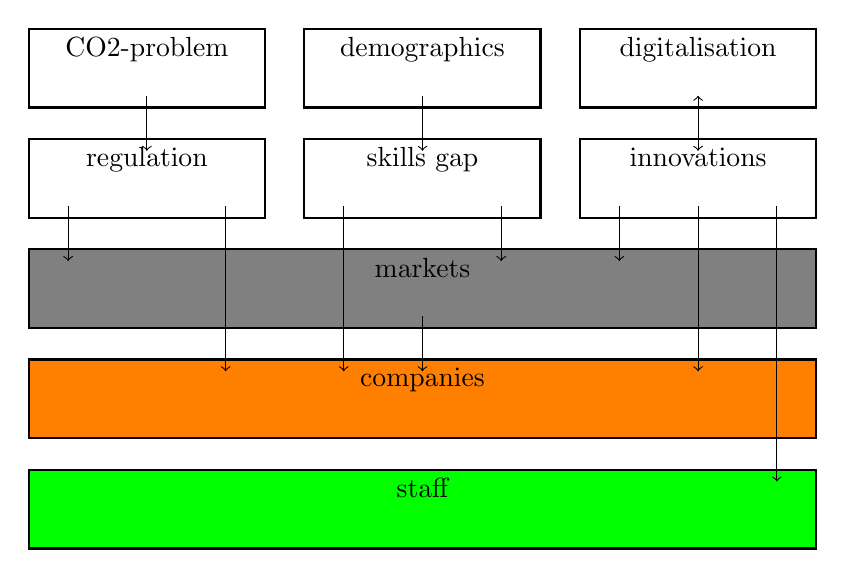
\begin{tikzpicture}[yscale=0.7]
    \def\smallbl{30mm}
    \def\bigbl{100mm}
    \node (co2p) [rectangle, draw, thick, minimum width=\smallbl, minimum height=10mm] at (-3.5,0) {};
    \node [below] at (co2p.north) {\ce{CO2}-problem};
    
    \draw[->] (-3.5,-0.5) -- (-3.5,-1.5);

    \node (ges) [rectangle, draw, thick, minimum width=\smallbl, minimum height=10mm] at (0,0) {};
    \node [below] at (ges.north) {demographics};
    
    \draw[->] (0,-0.5) -- (0,-1.5);
    
    
    \node (mang) [rectangle, draw, thick, minimum width=\smallbl, minimum height=10mm] at (0,-2) {};
    \node [below] at (mang.north) {skills gap};
    
    \node (digi) [rectangle, draw, thick, minimum width=\smallbl, minimum height=10mm] at (3.5,0) {};
    \node [below] at (digi.north) {digitalisation};
    
    \draw[<->] (3.5,-0.5) -- (3.5,-1.5);
    
    \node (regu) [rectangle, draw,   thick, minimum width=\smallbl, minimum height=10mm] at (-3.5,-2) {};
    \node [below] at (regu.north) {regulation};
    
    \node (inno) [rectangle, draw, thick, minimum width=\smallbl, minimum height=10mm] at (3.5,-2) {};
    \node [below] at (inno.north) {innovations};

    \node[fill=gray] (mark) [rectangle, draw, thick, minimum width=\bigbl, minimum height=10mm] at (0,-4) {};
    \node [below] at (mark.north) {markets};
    
    \node[fill=orange] (unte) [rectangle, draw, thick, minimum width=\bigbl, minimum height=10mm] at (0,-6) {};
    \node [below] at (unte.north) {companies};    

    \node[fill=green] (pers) [rectangle, draw, thick, minimum width=\bigbl, minimum height=10mm] at (0,-8) {};
    \node [below] at (pers.north) {staff};        

    \draw[->] (1,-2.5) -- (1,-3.5);
    \draw[->] (-1,-2.5) -- (-1,-5.5);

    \draw[->] (-4.5,-2.5) -- (-4.5,-3.5);
    \draw[->] (-2.5,-2.5) -- (-2.5,-5.5);
    
    \draw[->] (2.5,-2.5) -- (2.5,-3.5);
    \draw[->] (3.5,-2.5) -- (3.5,-5.5);
    \draw[->] (4.5,-2.5) -- (4.5,-7.5);

    \draw[->] (0,-4.5) -- (0,-5.5);

    % \node[right] (con) [rectangle, rounded corners, draw, thick, minimum height=10mm] at (6,-6) {Berater};

    % \draw[<->] (0,-6.5) -- (0,-7.5);

    
    % \node[right] (con) [rectangle, rounded corners, draw, thick, minimum height=10mm] at (6,-8) {Lehrer};
    
    % \node (banb) [rectangle, draw, thick, minimum height=30mm] at (9.5,-7) {Bildunganbieter};
        
    % \draw[->,dashed] (4.75,-7.5) -- (4.75,-2.5);
    
   % \draw[->,bend right=15] (co2p.west) to (pers.west);
    
    \end{tikzpicture}
\end{document}